% !TeX root = ../../thesis.tex
\chapter{Introduction}\label{ch:introduction}

\section{Semiconductor Image Sensors}

Photography is a ubiquitous commodity in modern life, with applications ranging from art and entertainment to science and space exploration, as well as surveillance and quality control. The inception of this technology is set in 1814, when the french inventor Joseph Nicéphore Niépce used a process called heliography to capture the first permanent photographic image. A few decades later, the more commonly known roll-film camera was patented by George Eastman, making photography more accessible to the public.

The digital imaging era starts in the middle of the 20th century, following the establishment of the semiconductor industry through the invention of the transistor. It began with the development of the charge-coupled device (CCD), which dominated the photography market until the 1990s, when complementary metal-oxide-semiconductor (CMOS) image sensors emerged. A CMOS image sensor (CIS) consists of several layers, including the microlens array, the color filter array (CFA), the photodiode, as well as the active pixel sensor (APS) circuitry. The role of each component can be summarized as following: (i) the microlens array consists of small lenses that collect and focus light onto light-sensitive areas of the sensors, (ii) the CFA consists of a mosaic of color filters that separate incoming light into red, green, and blue components, (iii) the photodiode is a silicon-based detector that converts light to electron-hole pairs, and lastly (iv) the APS circuitry, consists of multiple transistors that provide gain or buffer of the electrical charge from the photodiode.


The cost-effective, large-scale production of CMOS imagers in standard foundries, combined with their superior efficiency in power consumption and high-speed readout, has solidified their dominance in the photography market. Innovation continues to push boundaries, driving advancements in sensitivity, resolution, and compactness. Fig.~\ref{fig:ch1:pixel_size} highlights the advancement in pixel size and the efforts for continuous shrinking of the pixel size, getting close to surpassing resolutions of 576 Megapixel, which is the resolution of human eyes. The following section will highlight the challenges in this way, as well as the ways to mitigate those. 


\begin{figure}
  \centering
  \medskip
  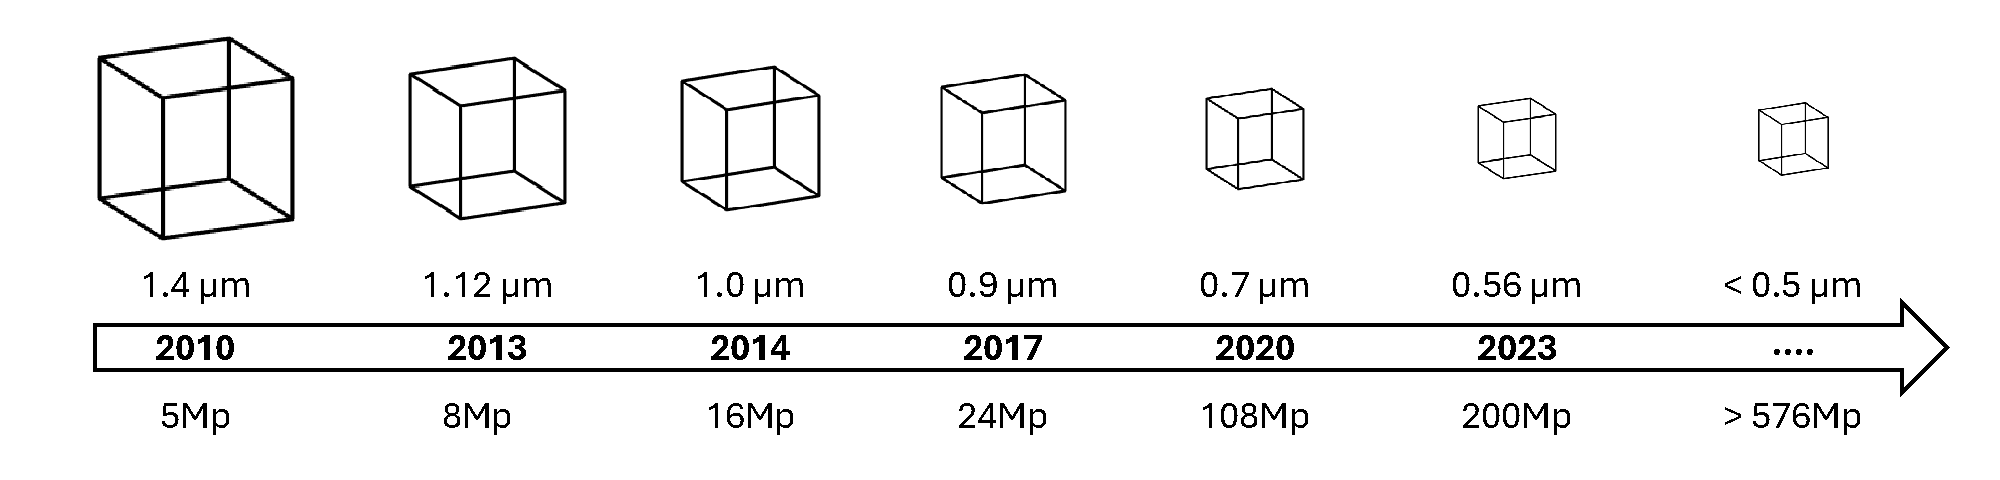
\includegraphics[width=.99\textwidth]{chapters/introduction/image/pixel_miniaturization.pdf}
  \caption[Short caption for Table of Figures]{Pixel miniaturization road map, Adapted from: \cite{SookyoungRoh2025Dispersion-engineeredSensors}}
  \label{fig:ch1:pixel_size}
\end{figure}

\section{Towards Ultra-High Resolution Imagers}

The drastic progress towards ultra-high resolution imagers has been propelled by multiple breakthroughs in semiconductor technologies, including (but not limited to) stacked device integration and photodetector separation. Stacked device integration is an advanced packing approach that entails the vertical integration of pixel, logic, and analog-to-digital converter modules, effectively reducing the footprint of the CIS circuitry. This advancement was initially attributed to the through-silicon-via (TSV) technology and more recently to the Cu-Cu direct bonding technology, as illustrated in Fig.~\ref{fig:ch1:stacking_technologies} \cite{Kagawa20193DSensors}. On the Si photodiode level, miniaturization has been accelerated with the introduction of electrical and optical separation be means of deep trench isolation (DTI). This process involves the etching of the area between two neighboring photodiodes and the its filling with materials including \ch{SiO_2}, poly-Si or tungsten, effectively reducing pixel crosstalk \cite{Ahn2014AGate, Okawa2019ALevel, Kim2020ATechnology, Park20217.9Isolation}.   

\begin{figure}
  \centering
  \medskip
  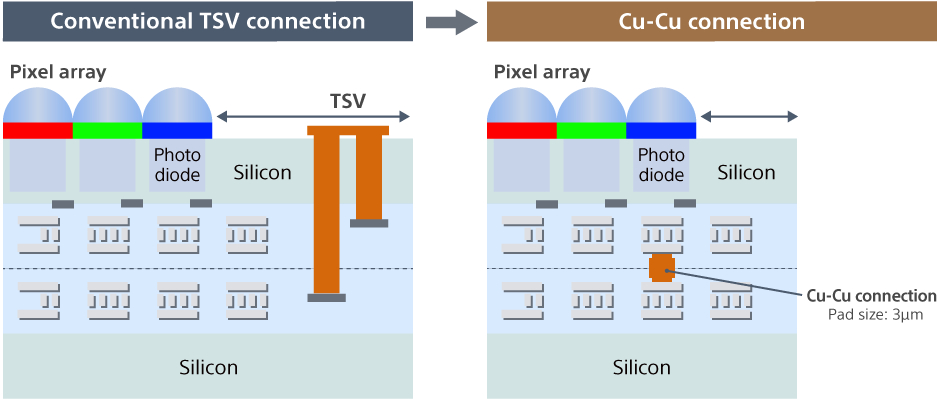
\includegraphics[width=.8\textwidth]{chapters/introduction/image/stacking.jpg}
  \caption[Short caption for Table of Figures]{Stacking technologies, Source: SONY}
  \label{fig:ch1:stacking_technologies} 
\end{figure}



However, the shrinking of the pixel size sets limitations to the detector's light sensitivity, considering that amount of photons that can be detected is proportional to the square of the pixel size \cite{Kim2024FreeformSensors}. The signal-to-noise ratio (SNR) is further exacerbated by the use CFAs, such as the Bayer pattern, which allows the transmittance of only one-third of the incident visible light spectrum. This limitation has lead to the development of alternative technologies for color sensing, which rely on color splitting rather than color filtering. These technologies rely on the use of waveguides or metasurfaces, with their concept illustrated in Fig.~\ref{fig:ch1:color_routing_concept}   \cite{Nishiwaki2013EfficientSensors, Miyata2019High-SensitivityMetasurfaces, Kim2024FreeformSensors, Zou2022Pixel-levelMetasurfaces, Catrysse2022SubwavelengthEfficiency}. However, these technologies are diffraction-based, meaning that they cannot be implemented for resolutions close or beyond the Abbe limit \cite{Shramkova2024HighSeparation}. It was recently demonstrated that this limitation can be overcome with the use a multimode color-splitting waveguide that utilizes the beating pattern of the interference between a symmetric and an asymmetric mode \cite{Kang2023Wafer-level-integratedSplitters}. The inception of this technology opened the way for achieving pixel pitch in the range of 0.2 $\mu m$ and is the main motivation of the work presented in the framework of this thesis. 


\begin{figure}[htbp]
    \centering
    % First plot
    \begin{subfigure}[t]{0.49\textwidth} % Adjust width as needed
        \centering
        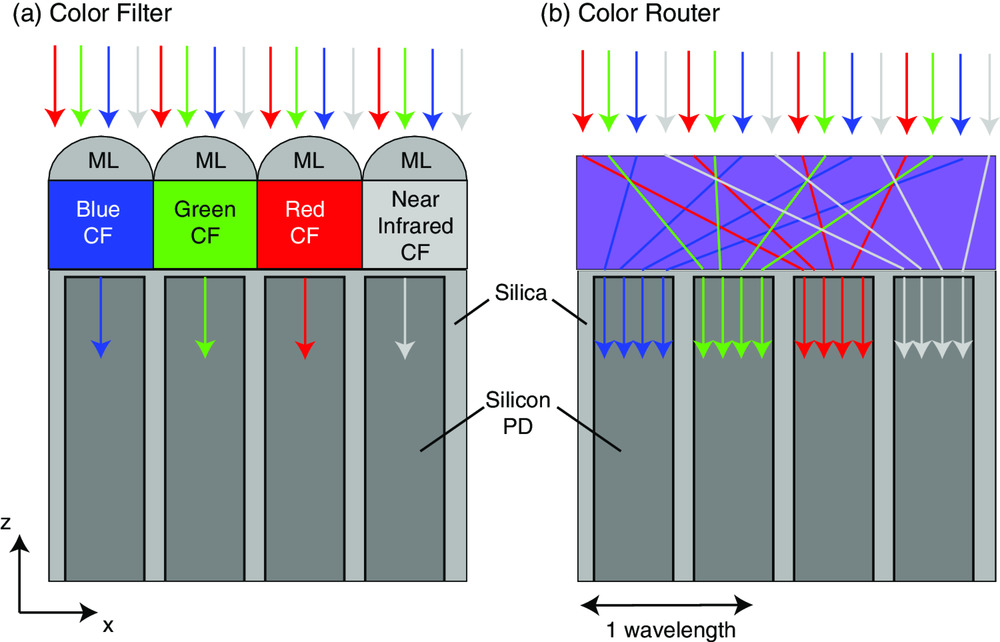
\includegraphics[width=\textwidth]{chapters/introduction/image/color_router.jpg} % Replace with your image
        \caption{}
        \label{fig:ch1:color_routing_concept}
    \end{subfigure}
    \hfill % Space between the two plots
    % Second plot
    \begin{subfigure}[t]{0.49\textwidth} % Adjust width as needed
        \centering
        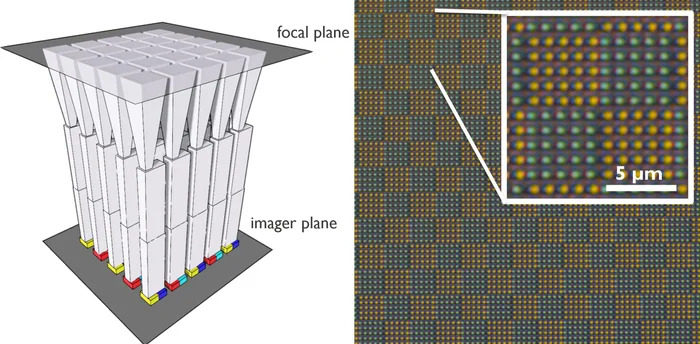
\includegraphics[width=\textwidth]{chapters/introduction/image/gigapixel_waveguide.jpg} % Replace with your image
        \caption{}
        \label{fig:ch1:gigalixel:waveguide}
    \end{subfigure}

    % Caption for the whole figure
    \caption{Perovskite phases and free energy: (a) Reproduced from \cite{Zhao2021PerfectPixels} (b) Reproduced from \cite{Kang2017HighCsPbBr3}.}
    \label{fig:ch1:color_splitting}
\end{figure}


\section{Beyond Silicon Photodiodes}

Amid rapid advancements in 3D stacking, pixel isolation, and color routing techniques, enhancing the performance of silicon photodiodes has become increasingly imperative. Their performance is largely governed by a well-known trade-off between absorption efficiency and response speed—a limitation primarily due to silicon's relatively low absorption coefficient for red wavelengths (> 620 nm). Typically, the photodiode thickness is in the range of 6 $\mu m$, imposing difficulties in achieving sub-microsecond response \cite{Han2016ASensors}. Additionally, the proposed color splitting technology could, in principle, enable the development of photodiodes with pixel pitch as small as 0.2 $\mu m$. However, such miniaturized structures are increasingly vulnerable to electrical and optical cross-talk, and fabricating DTI structures with such high aspect ratios becomes a non-trivial challenge. 

% More Si disadvantages from Ollearo thesis 

These limitations have sparked interest for introducing a deferent detector material with higher absorption coefficient in combination with the Silicon readout integrated circuit (ROIC). Such materials involved germanium (Ge) or III-V semiconductors, such as indium gallium arsenide (InGaAs). Haven't these materials have not shown promise for down scaling. Another option for visible light detection has been explored organic photodiodes, which however are characterized by lower mobilities due to their bulk heterojunction structure. This points attention to an emerging class of materials, that have gained immense attention for their use in optoelectronic applications. Perovskites. 


\section{Perovskite-Based Photodiodes}

\subsection{Properties of Perovskites}

\begin{figure}[htbp]
    \centering
    % First image (top)
    \begin{subfigure}[b]{\textwidth}
    \centering
        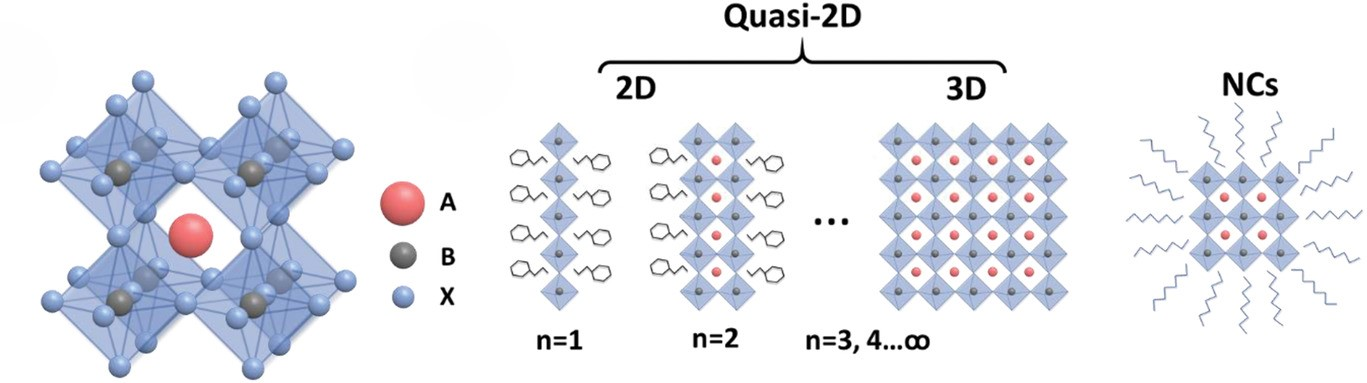
\includegraphics[width=0.85\linewidth]{chapters/introduction/image/perovskite_structure.jpg}
        \caption{}
        \label{fig:ch1:perovskite structure}
    \end{subfigure}

    \vspace{0.5cm}
    
    % Second image (bottom)
    \begin{subfigure}[b]{\textwidth}
    \centering
    %\hspace{-1.4cm}
        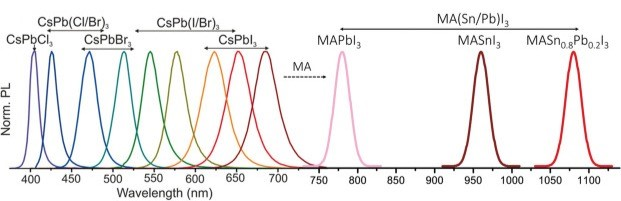
\includegraphics[width=0.85\linewidth]{chapters/introduction/image/bandgap_tunability.jpg}
        \caption{}
        \label{fig:ch1:bandgap_tunability}
    \end{subfigure}
    
    \caption{(a) Reproduced from \cite{Lei2021MetalApplications}. (b) Reproduced from \cite{Gholipour2020BandgapMaterials}.}
    \label{fig:ch1:perovskite_strucutre_bandgap}
\end{figure}



The term perovskite was first used in 1839 to name the newly discovered naturally occurring mineral calcium titanate (\ch{CaTiO_3}), but it took 170 years before perovskites were integrated into photovoltaic devices by the Miyasaka group in 2009 \cite{Kojima2009OrganometalCells}. Since then, intensive scientific research has enabled single-junction perovskite cells to surpass the power conversion efficiency (PCE) of the much more mature single-junction Si solar cells ($> 26\%$). Meanwhile, perovskite-Si tandem solar cells have demonstrated PCEs beyond the Shockley-Queisser limit ($>34\%$), establishing themselves as one of the most dominant candidates for next-generation solar technologies \cite{Hasan2024StabilityReview, Noman2024ATechnology}. This rapid growth of perovskite-based solar cell technology, from its inception to its commercial realization within 15 years, is attributed to both practical advantages and the exceptional optoelectronic properties of perovskites, as well. Practical advantages include, but are not limited to, low-cost production, dependence on abundant materials, and versatile fabrication through a wide variety of methods. On the other hand, some remarkable optoelectronic properties of perovskites are their tunable and direct bandgap, high absorption coefficient, low exciton binding energy, defect tolerance, and long carrier lifetime. 

\textbf{expand more on the advantages of perovskites - explain more and give metrics}

Perovskites can be divided into three groups, each of which has distinct properties: three-dimensional (3D), two-dimensional (2D) or quasi-2D, and zero-dimensional (0D) perovskites (Fig.~\ref{fig:ch1:perovskite structure}). 3D perovskites can be generally described by the \ch{ABX_3} formula, where A is a 12-fold-coordinated monovalent cation such as methylammonium (\ch{MA^+}), formamidinium (\ch{FA^+}), or cesium (\ch{Cs^+}), B is a 6-fold-coordinated inorganic divalent inorganic cation such as lead (\ch{Pb^{2+}}) and tin (\ch{Sb^{2+}}), while X is a strongly electronegative monovalent halide anion (\ch{I^-}, \ch{Br^-}, and \ch{Cl^-}). As a result, mixed compositions can be pursued for each lattice site, enabling the tuning of the perovskite's bandgap across a wide range of energies (spanning from near ultraviolet (UV) to near infrared (NIR)), depending on the desired application (Fig.~\ref{fig:ch1:bandgap_tunability}).

\subsection{From Solar Cells to Photodetectors}

The rapid advancements of perovskite-based solar cells sparked interest for their use in alternative optoelectronic applications, including photodiodes, light-emitting diodes (LEDs), and lasers. While solar cells operate without external bias, photodetectors typically operate in the reverse bias regime (to promote faster carrier extraction), while lasers and LEDs operate in the forward bias regime (to promote radiative charge recombination). While the diode structure is similar for all applications, the different operational regimes introduce distinct challenges for each use. Nevertheless, the operation of solar cells and photodiodes is more closely related, as they both depend on the efficient extraction of the photo-generated carriers. This process relies on the photovoltaic effect, during which the incoming light is absorbed by the active material, as long as its energy is equal or larger than the bandgap, leading to the generation of electron-hole pairs (or excitons). Under the effect of the built-in potential (which may be complimented by an additional field through reverse bias), the charge carriers are extracted and collected at the respective contacts as photocurrent. 

The solar cell structure, as well as the photodetectors that are developed in the framework of this thesis rely on the on the photodiode structure (Fig.~\ref{fig:ch2:types_of_detector}a), a vertical structure where the active layer is sandwiched between two charge transport layers, commonly referred to as the electron transport layer (ETL) and the hole transport layer (HTL). The role of these layers is typically twofold: (i) they promote the efficient extraction of the photo-generated carriers, and (ii) they block the injection of the opposite carrier from the electrode under the effect of reverse bias. The latter condition is only true for occasions where wide-bandgap transport layers are used. When developing the photodiode stack on top of a glass substrate, the architecture can be further distinguished in p-i-n and n-i-p, depending on the whether the perovskite is processed is processed on top of the HTL or ETL, respectively. 

The photodiode is not the only structure that is used for photo-detecting applications. Two additional types of photodetectors include the two-terminal photoconductors and the three-terminal phototransistors (Fig.~\ref{fig:ch2:types_of_detector}b and Fig.~\ref{fig:ch2:types_of_detector}c, respectively), which have both a lateral geometry. Both architectures rely on gain mechanism, which leads to a slower response time. At the same time, the relatively large spacing between the electrodes ($> 10 \mu m)$. not only requires a higher driving voltage but is also unsuitable for integration with readout circuits that have a significantly smaller pixel pitch (below 5 $\mu m)$.

\begin{figure}[htbp]
  \centering
  \medskip
  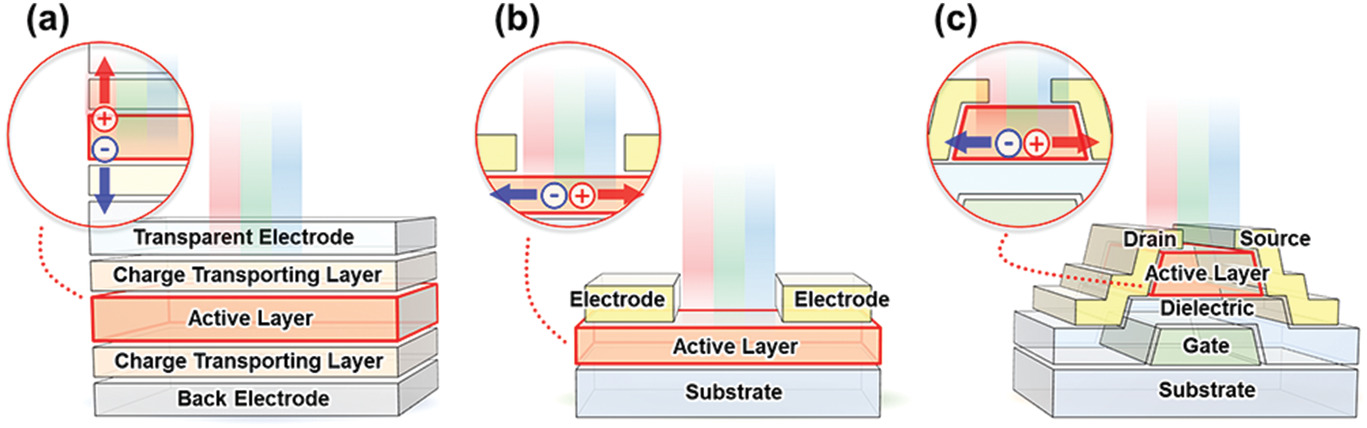
\includegraphics[width=.9\textwidth]{chapters/introduction/image/types_of_detector.jpg}
  \caption[Short caption for Table of Figures]{Photodiode, photoconductor, phototransistor, Reproduced from \cite{Yoo2021ADirections}.}
  \label{fig:ch2:types_of_detector}
\end{figure}

\subsection{Scalable, High-Temperature PePDs}



The vast majority of studies on perovskite-base optoelectronic devices rely on the use of solution processed methods, and specifically spin-coating. This is not surprising, considering that spin-coating is a technique that is simple, easily accessible, and has low cost. These characteristics make it highly suitable for rapid prototyping and exploration of various material combination that can promote efficiency or stability. For example, during solution preparation it is common to include various additives that in turn can help modulate morphology, optimize energy level-alignment or eliminate hysteresis \cite{Liu2020ACells}. However, cell fabrication through spin-coating is not transferable to industry, due to limitation is throughput and large-area deposition. For example, a commonly used technique, anti-solvent processing, has been shown to be challenging to scale-up \cite{Saki2021Solution-processedCells}.

\begin{figure}[htbp]
  \centering
  \medskip
  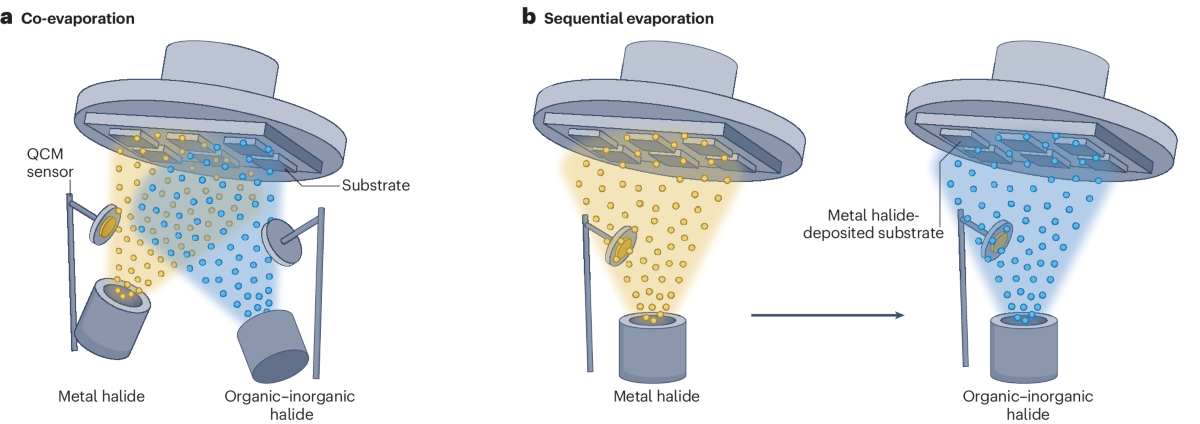
\includegraphics[width=.99\textwidth]{chapters/introduction/image/types_of_evaporation.png}
  \caption[Short caption for Table of Figures]{Types of evaporation: co-evaporation, single-source evaporation, sequential evaporation, Reproduced from \cite{Han2025PerovskiteCells}.}
  \label{fig:ch2:types_of_evaporation}
\end{figure}

Significant efforts have been made to explore alternative fabrication techniques that enable the scalable deposition of perovskite-based devices. Such methods involve solution-processed approaches (such as inkjet printing and spray coating) or vacuum-processed on (such as chemical vapor deposition or thermal evaporation). Among those, thermal evaporation is the most mature one, and in 2020 it enabled the fabrication of 21 $cm^2$ mini modules with the superior efficiency of 18.13\% \cite{Vaynzof2020TheProcessing, Li2020HighlyMini-modules}. Besides scalability, thermal evaporation offers the advantage of not necessarily requiring a post-deposition thermal annealing step, rendering highly attractive for applications that require the use of flexible substrates \cite{Becker2019LowExperimentation}. ON top of that, it avoids the use of toxic solvents, allows for precise control of the deposited thickness, and prevents the risk of damaging the underlying layers in tandem structures \cite{Zhang2020TowardCells, Forgacs2017EfficientCells}

Evaporation of perovskite thin films can be categorized into co-evaporation and sequential evaporation, as shown in Fig.~\ref{fig:ch2:types_of_evaporation}a and Fig.~\ref{fig:ch2:types_of_evaporation}b, respectively. Co-evaporation entails the simultaneous evaporation of the necessary precursors, rendering the careful monitoring and maintenance of evaporation rates ratio as highly crucial. On the other hand, in sequential evaporation each precursor is deposited individually, rendering the thickness of each layer as the defining parameter for the perovskites stoichiometry. Unlike co-evaporation, a post-deposition thermal annealing step is essential for sequentially deposited films to facilitate the reaction and intermixing of precursors, enabling the formation of the perovskite film. A third option for the evaporation of perovskite thin film, which is not illustrate, is the single-source evaporation. This approach requires an initial synthesis of the perovskite via powder mixing or crystal growth. Followingly, the powder mixture or the pulverized crystals are loaded in a single substrate from which they are evaporated. 


Despite the advantages of using thermal evaporation for the deposition of perovskite-based optoelectronic devices, several limitations still exist. For instance, the high vacuum pressure and low sticking coefficient of \ch{MA^+} renders its evaporation rather complicated \cite{Kim2020DepositionCH3NH3PbI3Perovskite}. At the same time, the inclusion of additives, which is crucial for improving the performance/stability of solution-processed films, is not compatible with evaporation. Lastly, evaporated perovskite films tend to have significantly smaller grain sizes, which may compromise their stability against moisture or limit device performance due to their higher defect density \cite{Vaynzof2020TheProcessing, Wang2017Scaling}.


Besides the use of spin-coating as the fabrication technique, research around perovskite optoelectronic devices is mainly focused on the use of hybrid organic-inorganic perovskites, where the A-site cation is a mixture of \ch{MA^+}, \ch{FA^+}, and/or \ch{Cs^+}, leading to optimal performances \cite{Zhang2021All-inorganicCells}. However, perovskites that contain organic molecules are more sensitive to thermal degradation. For instance, it was shown that methylammonium-based perovskites decompose into methylamine, hydrogen iodide, and lead iodide for temperatures beyond 100 \degree C. This limitation sets hybrid organic-inorganic perovskites unsuitable for applications with high thermal budget, which may be imposed by intrinsic (triggering of self-heating mechanisms through resistive loses) or extrinsic factors (high ambient temperature, high temperature post processing) \cite{Handa2019LargePerovskite, Dong2021SupportingFilm, Li2022StructureTemperatures}. Such a condition is imposed in the case of color-splitting waveguides, which have to be bonded to the underlying photodetector structure at temperatures beyond 200 \degree C. 

\begin{figure}[htbp]
    \centering
    % First plot
    \begin{subfigure}[t]{0.56\textwidth} % Adjust width as needed
        \centering
        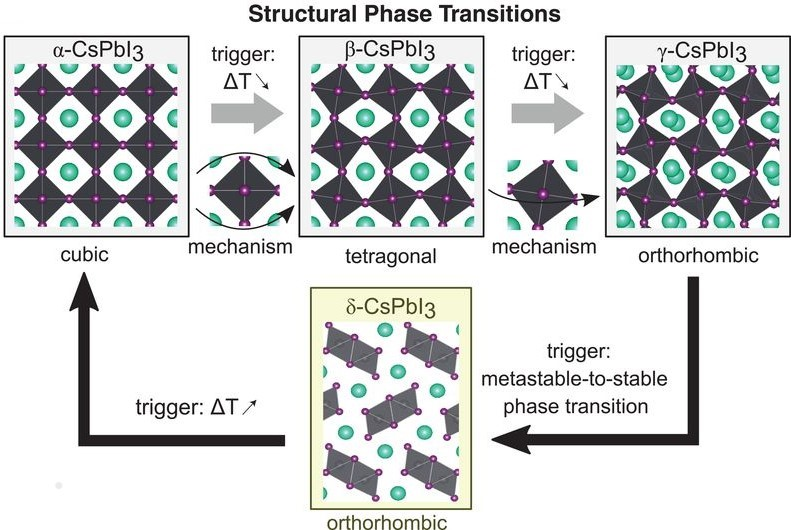
\includegraphics[width=\textwidth]{chapters/introduction/image/perovskite_phases.jpeg} % Replace with your image
        \caption{}
        \label{fig:ch2:perovskite_phases}
    \end{subfigure}
    \hfill % Space between the two plots
    % Second plot
    \begin{subfigure}[t]{0.39\textwidth} % Adjust width as needed
        \centering
        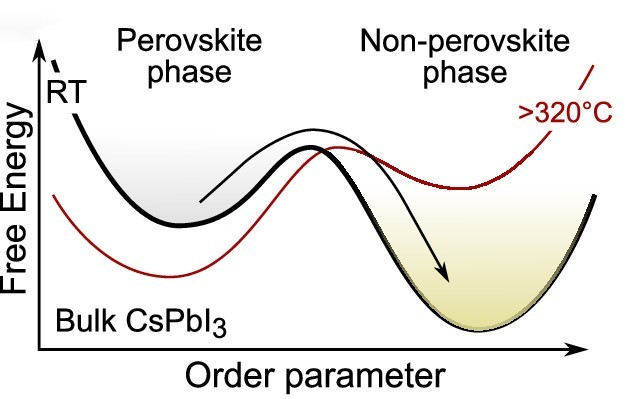
\includegraphics[width=\textwidth]{chapters/introduction/image/perovskite_free_energy.jpeg} % Replace with your image
        \caption{}
        \label{fig:ch2:perovskite_free_energy}
    \end{subfigure}

    % Caption for the whole figure
    \caption{Perovskite phases and free energy: (a) Reproduced from \cite{Steele2019ThermalFilms} (b) Reproduced from \cite{Steele2021TrojansPerovskite}.}
    \label{fig:ch2:phases_and_free_energy}
\end{figure}

Under these circumstances, all-inorganic perovskites, in the \ch{CsPbI_{x}Br_{3-x}} ($0 \le x \le 3$) family become an attractive solution, since they have been proven to withstand temperatures beyond 250 \degree C \cite{Dong2021High-TemperatureCells}. The two endmembers of this composition are \ch{CsPbI_3} and \ch{CsPbBr_3}. The latter has a bandgap close to 2.3 eV ($\sim$ 540 nm), which is unsuitable for visible light detection, considering that it completely excludes the red part of the spectrum \cite{Tong2020RecentCells}. On the other hand, \ch{CsPbI_3} has a reported bandgap in the range of 1.7 eV, allowing for the detection of the complete visible light spectrum \cite{Zhao2018ThermodynamicallyPhotovoltaics}. However, \ch{CsPbI_3} exists in several phases, and the photoactive (black) phases are only stable in elevated temperatures. In room temperature, a yellow, non-perovskite phase ($\delta-$ \ch{CsPbI_3}) with significantly larger bandgap (~2.8 eV) is the thermodynamically preferred one, rendering it unsuitable for any kind of optoelectronic application \cite{Cho2021Long-termNetwork, Burwig2018CrystalFilms, Steele2022AnFilms}. The black phase consists of the $\gamma-$ (orthorhombic), $\beta-$ (tetragonal), and $\alpha-$ (cubic) phase, which are similar in structure and properties and emerge beyond 320 \degree C. It is possible to kinetically trap the black phase at room temperature through rapid cooling, however the yellow phase re-emerges almost instantaneously when the perovskite film is exposed to ambient moisture \cite{Steele2019ThermalFilms}. 

To develop a better understanding of the stability or perovskite films and ways to enhance it, it is important to introduce a few new parameters, namely the tolerance factor (t), the octahedral factor ($\mu$), and the atomic packing fraction ($\eta$). The tolerance factor, defined as:
\begin{equation}
    t = \frac{r_A + r_X}{\sqrt{2}(r_B + r_X)},
\end{equation} 

where $r_A$, $r_B$, and $r_X$ are the ionic radius of the A, B, and X sites, respectively \cite{Goldschmidt1926DieKrystallochemie}. A perovskite can be formed for $0.8 < t < 1.0$, where $t = 1$ represents an ideal cubic perovskite. The octahedral factor represents the ratio between the radii of the B-site cation and the X-site anion ($\mu = r_B/r_X$), while the atomic packing factor (APF) describes the fraction of a crystal structure's total volume that is occupied by its constituent atoms. Using this parameters, Sun et al. introduced a stability descriptor ($(\mu + t)^2$), that can predict the relative stability between two perovskites and is visualized in Fig.~\ref{fig:ch2:perovskite_stable_region} \cite{Sun2017ThermodynamicPerovskites}. Taking the computational error into account, it can be seen that the \ch{CsPbI_3} composition is on the borderline between the stable and non-stable region, explaining its metastable behavior at room temperature.  

\begin{figure}[htbp]
  \centering
  \medskip
  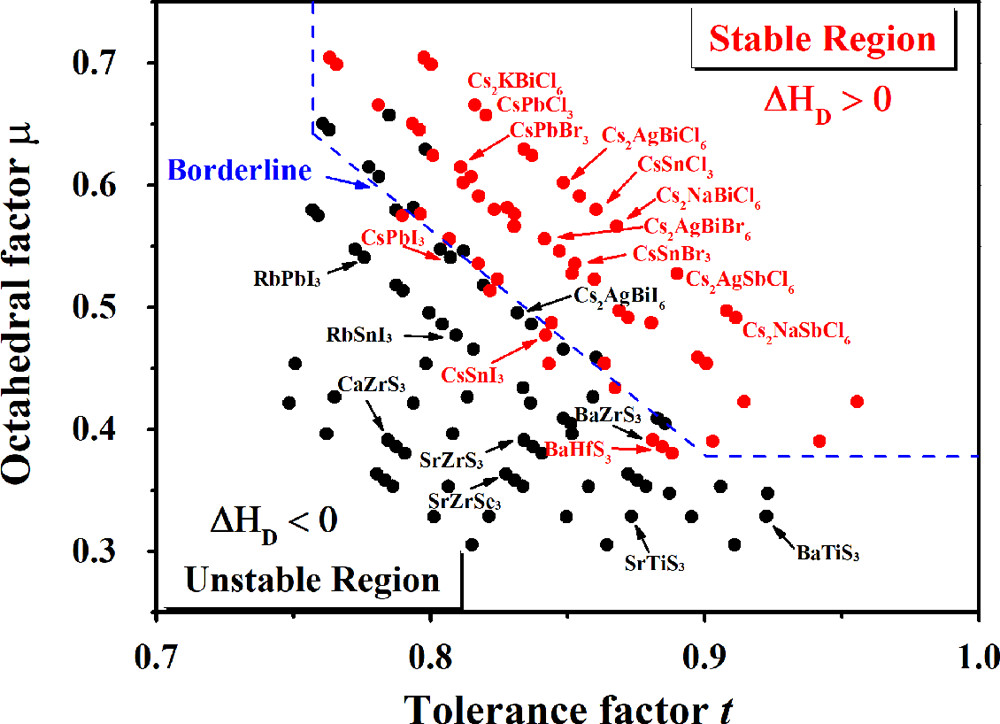
\includegraphics[width=.67\textwidth]{chapters/introduction/image/perovskite_stability.jpeg}
  \caption[Short caption for Table of Figures]{Region of perovskite stability, Reproduced from \cite{Sun2017ThermodynamicPerovskites}.}
  \label{fig:ch2:perovskite_stable_region}
\end{figure}

Several strategies have been explored to enhance the stability of\ch{CsPbI_3} in ambient conditions, including component engineering, additive engineering, dimensionality reduction engineering and phase mixing engineering \cite{Lei2024StabilityPerovskites}. There are also mechanical approaches, such as such as the pressure-assisted tuning of the \ch{[PbI_6]^{4-}} octahedra tilting \cite{Ke2021PreservingTilt} or the pattering of the perovskite film with a \ch{PbI_2} microgrid via laser writing \cite{Steele2022AnFilms}. Expand a bit more on these options...

Component engineering, achieved through the partial replacement of the A-, B-, or X-site, enables composition shifts toward the stable region of Fig.~\ref{fig:ch2:perovskite_stable_region}, while maintaining compatibility with thermal evaporation and avoiding the use of organic compounds. This effect can be achieved by partially replacing \ch{I^-} with \ch{Br^-}. The latter has a smaller ionic radius, effectively increasing the crystal's tolerance factor. However, a trade-off between stability and bandgap suitability arises, considering that \ch{CsPbBr3} is transparent for the red part for the visible spectrum. A reasonable compromise is reached with \ch{CsPbI_2Br}, with a bandgap in the range of $\sim$ 1.95 eV. Such a composition can be easily achieved via the co-evaporation of CsBr and \ch{PbI_2} powders in a 1.00:1.00 molar ratio. 


A variety of reports have employed the \ch{CsPbI_2Br} composition for the fabrication of solar cells and photodiodes, including deposition via thermal evaporation. However, in all cases the perovskite was combined with solution-processed and/or organic transport layers, which counterbalances the advantages of using a vacuum-deposited, inorganic active layer. In fact, besides a report previously published within our group \cite{PintorMonroy2021All-EvaporatedApplications}, and to the best of our knowledge, there is truly limited number of reports that have produced all-inorganic, vacuum-deposited perovskite optoelectronic devices. 


\section{Scope and Aim of This Thesis}

\subsection{Performance Metrics}

The definition of performance metrics for any device depends on its intended application. In our case, this is translated into the integration of the PePD on top of a silicon readout integrated circuit (ROIC), as well as the bonding of the structure with the color-splitting waveguides. The former mainly defines the metrics related to electrical performance, while the latter defines the metrics related to stability. 


\begin{figure}[htbp]
    \centering
    % First plot
    \begin{subfigure}[t]{0.55\textwidth} % Adjust width as needed
        \centering
        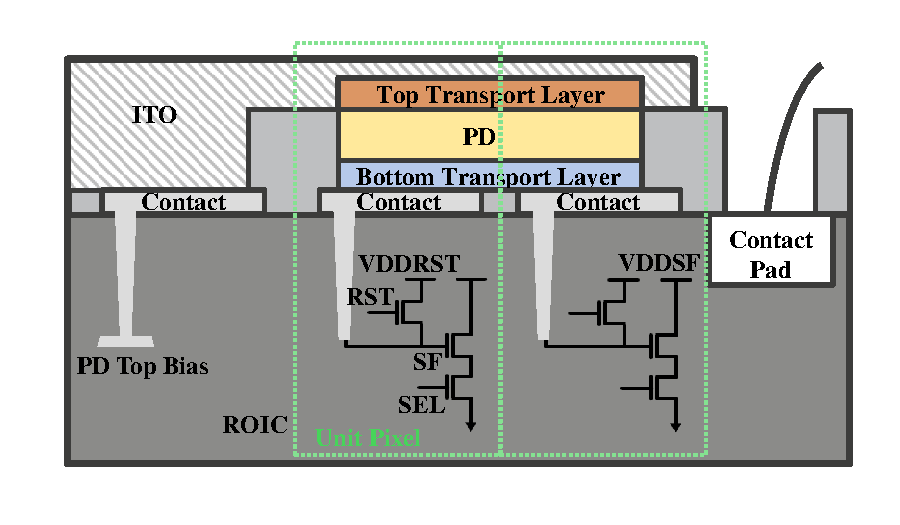
\includegraphics[width=\textwidth]{chapters/introduction/image/imager_cross_section.pdf} % Replace with your image
        \caption{}
        \label{}
    \end{subfigure}
    \hfill % Space between the two plots
    % Second plot
    \begin{subfigure}[t]{0.99\textwidth} % Adjust width as needed
        \centering
        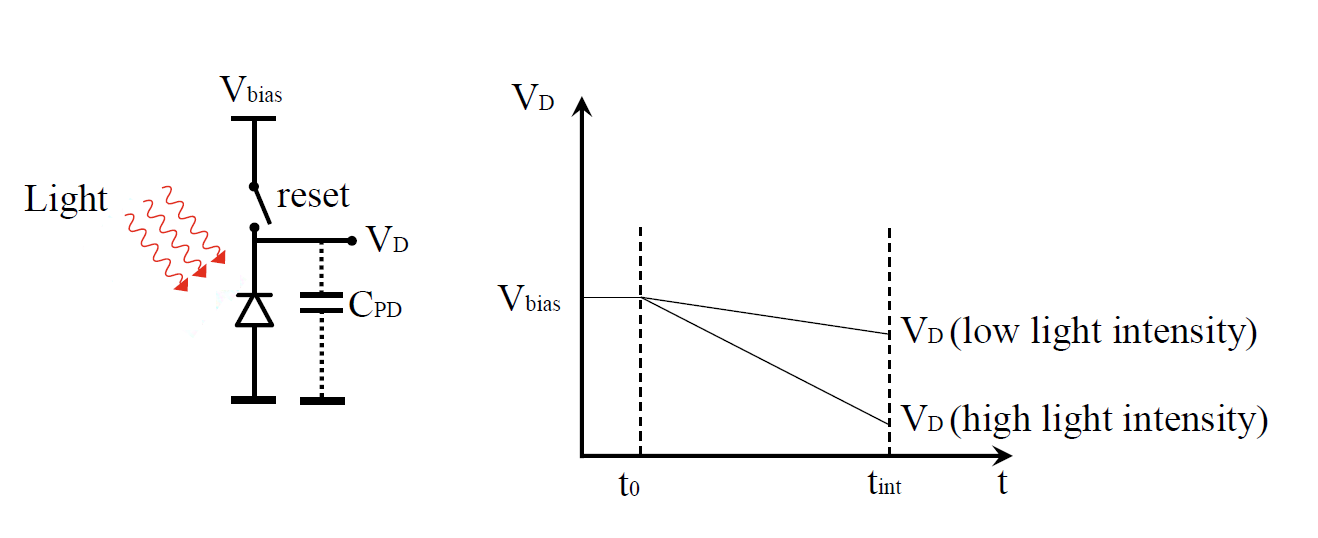
\includegraphics[width=\textwidth]{chapters/introduction/image/3T_pixel_readout.png} % Replace with your image
        \caption{3T pixel readout, Reproduced from \cite{Pejovic2023ColloidalInfrared}.}
        \label{}
    \end{subfigure}

    % Caption for the whole figure
    \caption{}
    \label{fig:ch1:cmos_roic}
\end{figure}



For a better understanding of the metrics stemming from the CMOS integration, a better understanding of the readout mechanism is crucial. In our case, this mechanism relies on the 3T pixel design, which involves the photodiode and three additional transistors, namely the reset, the source follower and the row select transistor. This schematically illustrated in Fig.~\ref{fig:ch2:readout}. A read-out cycle is defined by the duration of the  integration period ($t_{int}$). At the beginning of the integration period ($t_0$), the reset transistor is briefly turned-on, connecting the photodiode to a reference voltage in the reverse regime ($V_{bias}$). Next, the reset transistor is turned-off, however $V_{bias}$ is maintained across the photodiode, due to its internal capacitance ($C_{PD}$). During the integration period, and with the photodiode under illumination, the absorbed photons are converted to electron-hole pairs, which in turn discharge the diode's internal capacitance, effectively reducing the bias across its terminals. As a result, at the end of the integration period, the bias across the diode is $V_D$, whose value depends on the number of absorbed photons, i.e. the light intensity. Lastly, $V_D$ is buffered by the source follower transistor and read by the rest of the circuit. 

The performance should be reliable across the voltage swing (100s mV to 1 V), therefore we consider the operation region up to -2 V. This is in contrast to most reports farbicating and cahracterizing perovskite-based photodiodes, which limit the operatioal scope up to -0.5 V.

This procedure help us evaluate the performance of the photodiode according to the following criteria: 

\textbf{Dark Current Density:}

One of the most critical factors that indicates the performance of photodetectors is the dark current density (Jd), which constitutes the primary limitation on the device’s detectivity. Previous reports have shown that careful optimization of the ETL and HTL is critical for minimizing Jd in perovskite-based photodetectors. This was achieved by eliminating shunt pathways25, increasing the carrier injection barrier26,27, and preventing interfacial thermal charge generation28,29. However, most reports typically restrict the operational voltage range to approximately -0.5 V, despite the potential for higher carrier extraction speeds at greater reverse biases. This is because extensive reverse biasing of perovskite heterojunctions is known to have adverse effects on the device performance, including the risk of device breakdown. This manifests as a multiple-orders-of-magnitude increase in Jd and has been attributed to the creation of defect states in the perovskite bulk that act as charge recombination centers30. 

\textbf{External Quantum Efficiency:}
High and saturated across the voltage swing (100 ms to 1 V)

\textbf{Responsivity and Specific Detectivity}

\textbf{Linearity:}

\textbf{Response Speed:}

\begin{itemize}
    \item Develop an all-inorganic perovskite diode (many reports use inorganic perovskites with organic TLs - this defies the purpose of using an inroganic absorber)
    \item Evaluate the deposition conditions on performance and repeatability of the photodetector
\end{itemize}


%%%%%%%%%%%%%%%%%%%%%%%%%%%%%%%%%%%%%%%%%%%%%%%%%%
% Keep the following \cleardoublepage at the end of this file, 
% otherwise \includeonly includes empty pages.
\cleardoublepage

% vim: tw=70 nocindent expandtab foldmethod=marker foldmarker={{{}{,}{}}}
